\documentclass{article}

\begin{document}
	\section{Model}
	
	

\subsection{Model and Parameter selection}

In order to proceed this reaction-diffusion system for VMC pattern formation process, Alan Garfinkel and his partners made the following choices. The first choice is that they treated this model as 2D spatial domain in 100*100 uniform mesh. Meanwhile the activator and inhibitor are BMP-2 and MGP corresponding to U(x,y) and V(x,y) (effective concentrations). The method to calculate the final concentrations for BMP-2 and MGP is the use of second order Runge-Kutta method. Moreover the chemical kinetics they chose were the interactions of BMP-2 with MGP. Additionally, in order to govern the model equations, the initial condition is described as following “The initial condition of U and V that are uniformly distributed with a 2\% random perturbations” as well as neumann conditions (no-flux at boundary) for their boundary conditions. The whole equations are the following:

In these above equations, D is the ratio of diffusion coefficient of BMP-2 and MGP which is $D_u / D_v$ (BMP-2 and MGP respectively). $\gamma$ is the scaling parameter which is equal to $\frac{L^2}{D_v T_C}$, where $L$ is the length of the domain which is the actual size in their experiments, $T_C$ is the time for BMP-2 synthesis. $k$ is the saturating value. $c$ and $e$ are the first order degradation rates for BMP-2 and MGP. $S$ is source term.

More precisely, in equation 1, BMP-2 will activate its own production autocatalytically which will saturate. Hence Garfinkel et al chose $\frac{U^2}{1+k U^2}$, a sigmoidal form, to govern this autocatalysis. V is treated as the inhibitor in the denominator. There is a degradation for U at rate c. In equation 2, $U^2$ is used to represent that BMP-2 spurs MGP in non-linear manner. There is a degradation for V at rate e. S represents the exogenous MGP which is added by purpose.

In order to run the equations smoothly, the parameters were chosen carefully. Firstly, Garfinkel et al took the initial value of $Du$, $1 \times 10^{-8} cm^2/sec$, directly from Entchev et al’s work which was calculated by using GFP labeling and imaging. Then they considered the diffusion of large amount of molecules in nonlinear slowing manner. Due to acid PH, dimerization of BMP-2 and actual tissue culture, the estimated value reduced to $0.15 \times 10^{-8} cm^2/sec$. Because there is no directly calculated value for diffusivity of MGP, they estimated an theoretical approximate value, $30 \times 10^{-8} cm^2/sec$, which was based on empirical formulas. Meanwhile, this approximate value is similar to the diffusion coefficient of amyloid B which is $50 \times 10^{-8} cm^2/sec$. Finally, the value of D was calculated by $\frac{D_u}{D_v} = \frac{1}{200}$.

In the previous experiment which was done by Ghosh-Choudhury et al, it shows that BMP-2 autoregulates in a saturating manner. However, due to unknown level of MGP, it is difficult to establish the precise value of k. In Garfinkel et al’s model, they chose k=0.65.

In order to calculate , it is essential that production rates are known. In previous work, they have found the upper limit for the production rate which is in embryonic kidney cells with a cytomegalovirus (CMV) promoter. They also established the rates for BMP-2 production in calcifying vascular cells and in endothelial cells which were both . Furthermore, FLAG-tagged MGP and newly developed ELISA suggested that the production rates of BMP-2 and MGP are similar. These reports can inform that the upper limit for the production rates is  and the lower limit is .

 As mentioned above,  is equal to . In the actual cell culture, the is 4cm,  they chose is 1 ng/hr (). Hence the 

Garfinkel et al estimated the degradation rate of BMP-2 directly and conservatively from the calculation of Entchev et al’s work. Hence they took c = 0.01. MGP has more rapidly degradation than BMP-2 based on their unpublished work. The ratio for  is approximately . Thus they took e = 0.02.

The source term S is to be added in order to make tripling pattern formation which means the source term needs to be three times the initial concentration of MGP. In the model, Garfinkel et al chose the initial value of MGP scaled as 2. Then for the 1000 time steps, the S needs to be 0.06 per time steps, totally 6 which will make tripling pattern formation.

\subsection{Non-dimensionalization and Steady States}

Using the scaling factors $u=\sqrt{k}U$, $v=c\sqrt{k}V$ as well as $\tau = \gamma c t$ and $\vec{\xi}=\sqrt{\gamma c} \vec{x}$ we were able to non-dimensionalize the system as
$$\frac{\partial u}{\partial \tau} = D\nabla^2 u + \frac{u^2}{(1+u^2)v}-u,\ \ \ \frac{\partial v}{\partial \tau} = \nabla^2 v + G u^2 - E v + Z$$
where $G=\frac{1}{\sqrt{k}}$, $E=\frac{e}{c}$ and $Z=\sqrt{k}S$.


The steady state at $(\bar u_0,\bar v_0)=(0,S/E)$ is apparent and quickly confirmed to stable. We found another stable steady state numerically, which suggests the existence of a third, unstable steady state.
This notion is corroborated in Garfinkel 2008 which additionally provides analytical forms of the non-trivial steady states. We were able to proof the equivalence of the two systems of equations and the analyses from the later paper can thus be applied to  our model. The stable (+) and unstable (-) steady states (for $G=1$, $k=1$, $E=2$) are

$$(u_\pm,v_\pm)=\Bigg(\frac{\sqrt{\theta}\pm\sqrt{\eta}}{2}, \frac{\theta\pm\sqrt{\theta\eta}}{2-(Z-1)\sqrt{\theta}\pm\theta\sqrt{\eta}}\Bigg)$$

where $\eta = \frac{4}{\sqrt{\theta}+\phi}$, $\theta=\frac{\beta/\rho-\rho-2(Z+1)}{3}$, $\phi = -\theta-2(Z+1)$, $\rho = \sqrt[3]{\alpha/2+\sqrt{\alpha^2/4-\beta^3}}$, $\beta = 1+14Z+Z^2$, $\alpha = 108-72Z(Z+1)+2(Z+1)^3$

\subsection{Stability and Bifurcations}

More interesting than the precise values of the steady states are their stabilities and how those change with parameter $Z$. In the last section we noted the existence of two stable and one unstable steady state: the system exhibits bistability. This is true for a limited range of $Z$ only as Garfinkel at al. describe in their 2008 article, in which they add a layer of analysis to study the systems bifurcations along the parameter $Z$ ($S$ in their nomenclature).

Garfinkel et al. add theoretical explanation for the range of patterns occuring at different intervals of the parameter space which we will not attempt to recapitulate. Importantly, equivalency between the two models requires that we are able to reproduce the results in Fig. 1 (adjusted by the scaling factor $1/\sqrt{k}$).


\begin{figure}[H]
\centering
  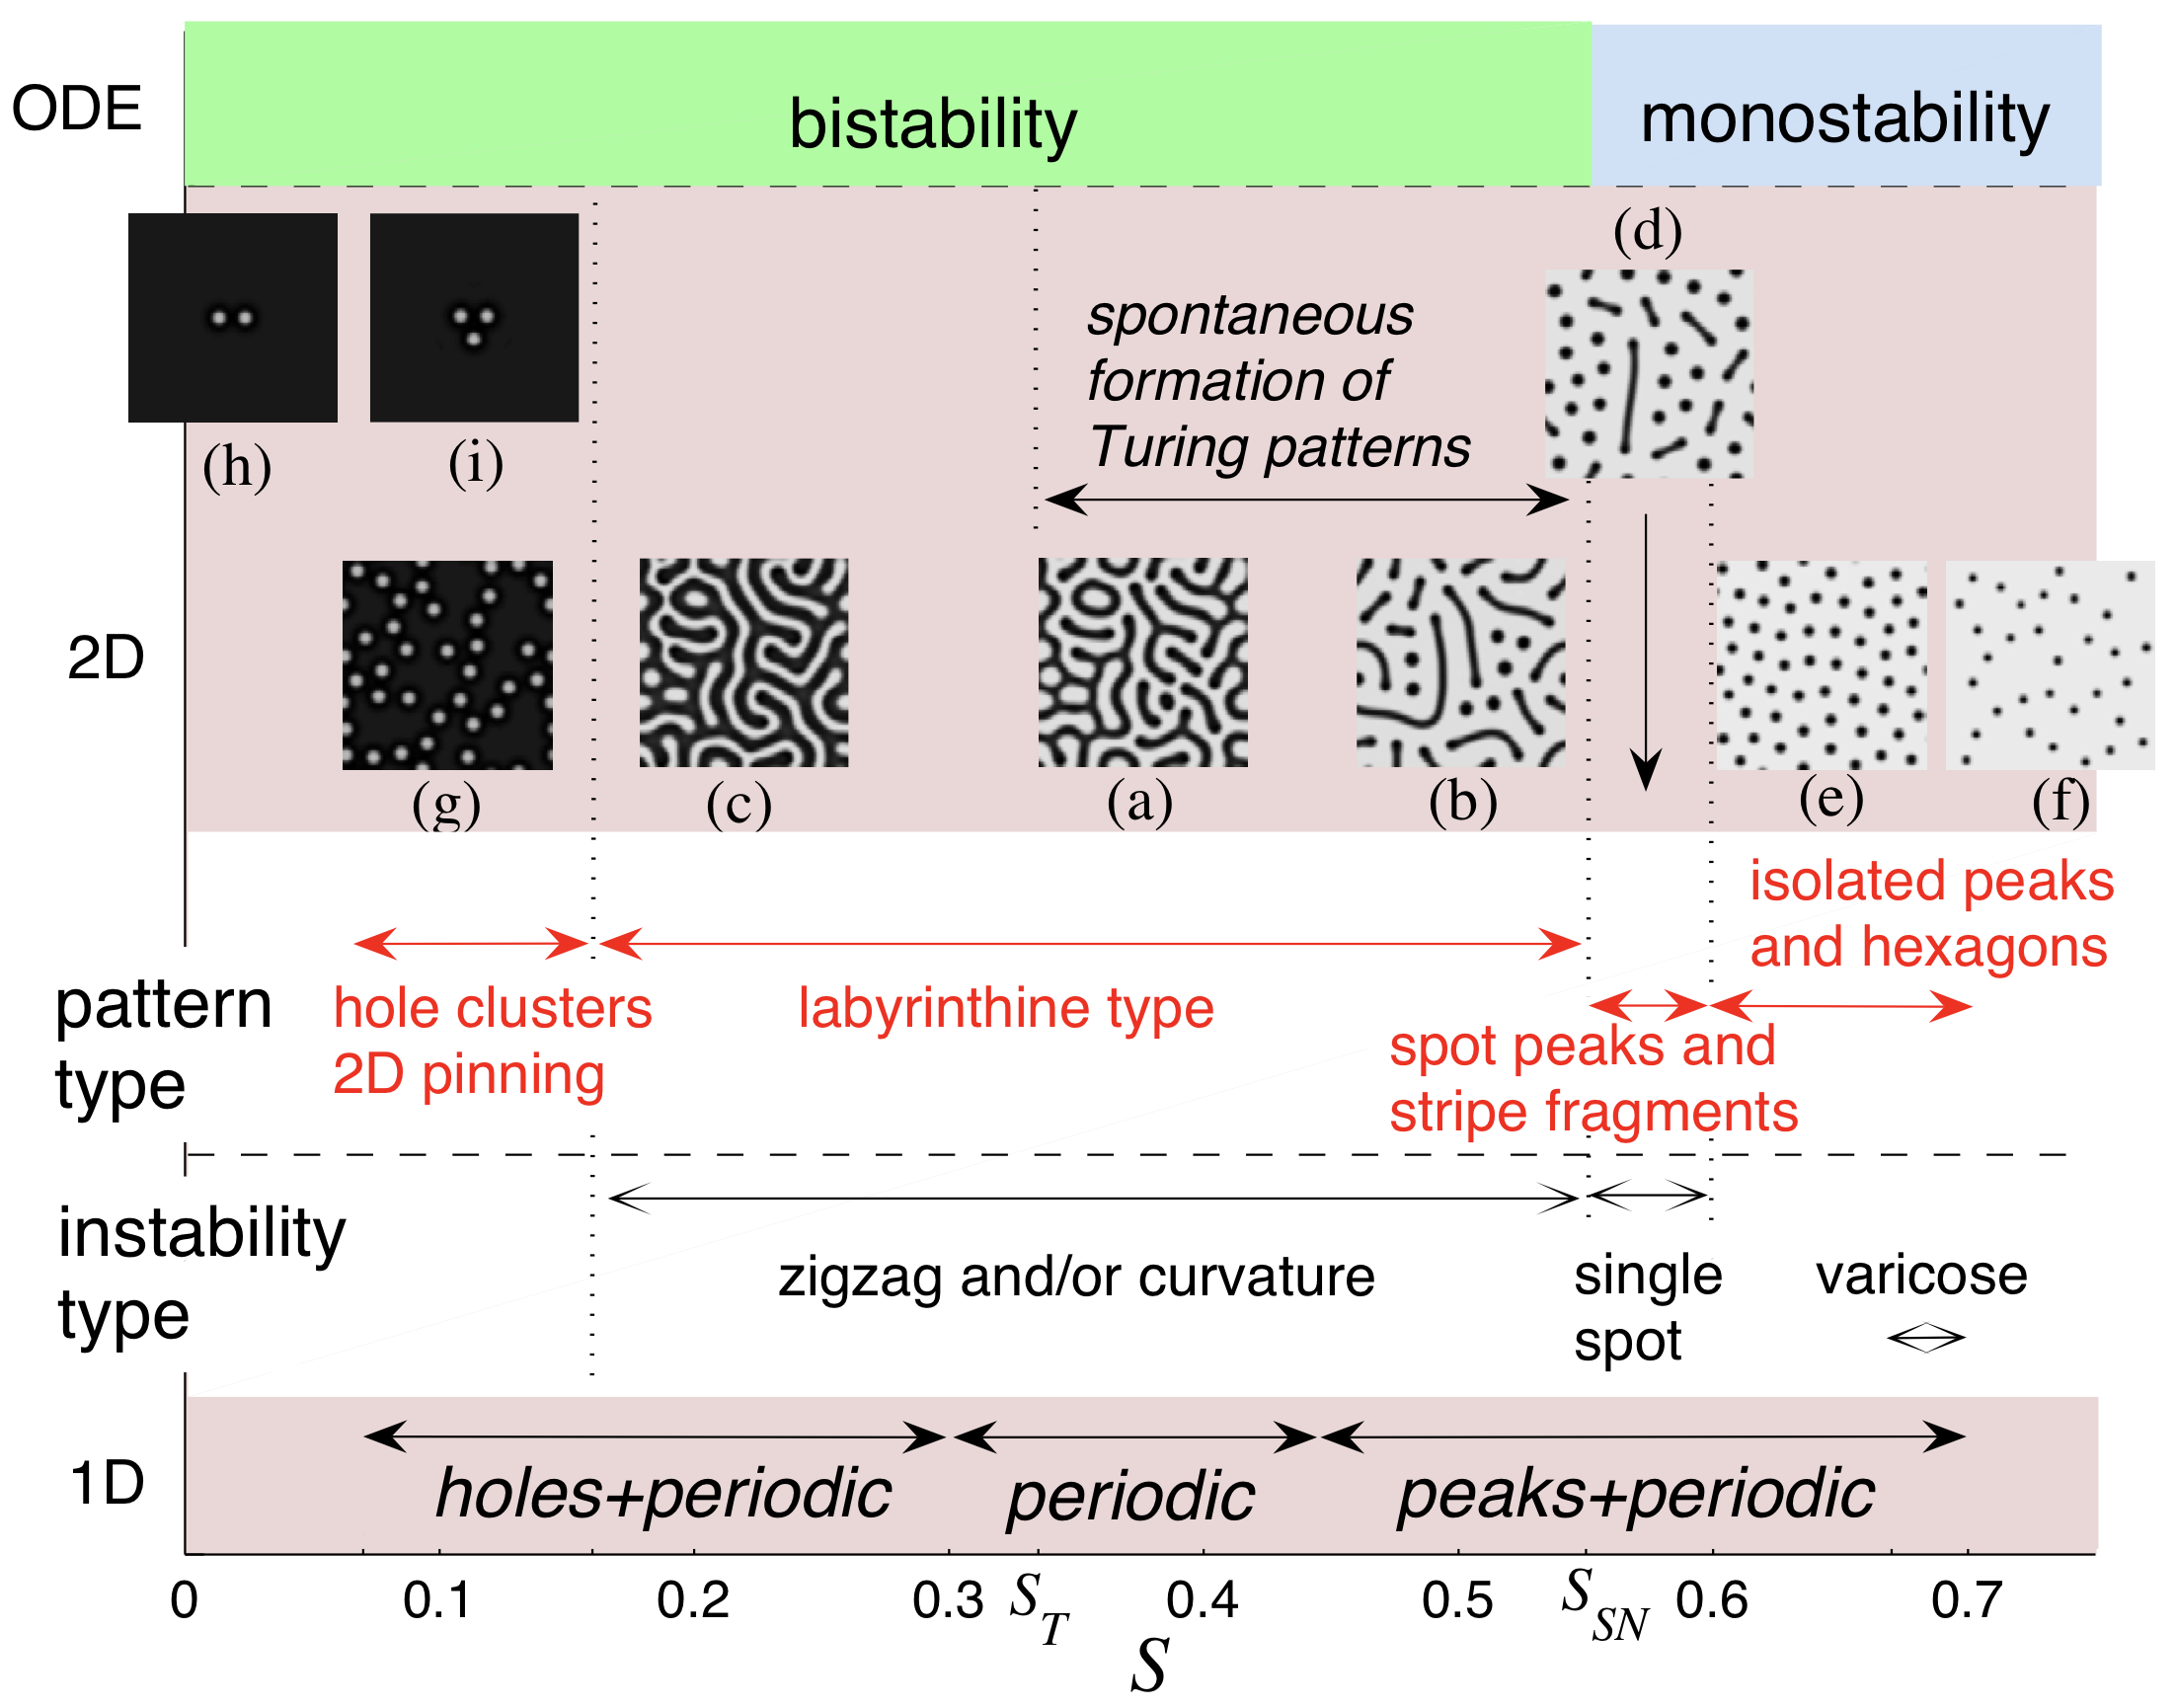
\includegraphics[width=0.7 \linewidth]{parameter_space.png}
  \caption{}
  \label{fig:s}
\end{figure}

Fig. 1 identifies four qualitatively different regions. [how and why?]



\end{document}